\documentclass[a4paper]{article}
\usepackage[utf8]{inputenc}
\usepackage[T1]{fontenc}
\usepackage{lmodern}
\usepackage{listings}
\usepackage{graphicx}
\usepackage{dirtree}
\usepackage{caption}
\usepackage{subcaption}
\usepackage{float}
\usepackage[english]{babel}
\title{Human Intracranial Brain Observations Player \\ User Manual}
\author{\textsc{BONTEMPS Benjamin} \\ \textsc{CHATARD Benoît} \\ \textsc{GANNERIE Adrien}}
\lstset{
	frame = single,
	basicstyle = \footnotesize\ttfamily
}

\begin{document}
\maketitle
\begin{abstract}
This document is the user manual of the Human Intracranial Brain Observations Player (HiBoP). HiBoP is being developed by the Centre de Recherche en Neurosciences de Lyon (CRNL), with funds from the Human Brain Project (HBP) to visualize large datasets of intracranial electroencephalography (iEEG) data. This document was written for the 2.1.0 version of HiBoP.
\end{abstract}
\tableofcontents
\section{HiBoP project} \label{data}
\paragraph{} A \textbf{Project} links together anatomical and functional data from a set of patients. If you have an anatomical description of the patients (3D mesh of the brain, MRI and coordinates of the sites of the electrodes) and the respective iEEG data, you can visualize them in 4D (3D space + time). The first thing to do with HiBoP is to create or open a Project. This can be done within HiBoP (section \ref{UI}), but also using a third-party software which automatically generates the files and the hierarchy, such as the HiBoP Database Manager (appendix \ref{bddmanager}).
\paragraph{} On your Hard Drive, the Project consists of a folder with several subfolders (Figure \ref{projectDirectory}). Each file in this subfolder is encoded with the json format, and thus can be edited (at your own risks) using any text editor. However this is not recommended, as any coma missing may cause the file to be incorrectly interpreted.
\begin{figure}[H]
\framebox[\textwidth]{%
\begin{minipage}{0.9\textwidth}
\dirtree{%
	.1 ProjectName/.
	.2 ProjectName.settings.
	.2 Datasets/.
	.3 DatasetName.dataset.
	.3 ....
	.2 Groups/.
	.3 GroupName.group.
	.3 ....
	.2 Patients/.
	.3 PatientName.patient.
	.3 ....
	.2 Protocols/.
	.3 ProtocolName.prov.
	.3 ....
	.3 Icons/.
	.4 Icon1.png.
	.4 Icon2.jpg.
	.4 ....
	.2 Visualizations/.
	.3 VisualizationName.visualization.
	.3 ....
}
\end{minipage}
}
\caption{\label{projectDirectory}Project directory hierarchy}
\end{figure}
\subsection{Settings}
\paragraph{} The .settings file at the root of the projet folder describes some project settings (Figure \ref{projectSettings}). This file contains a default path for the anatomical data of the patients and a default path for the functional data (iEEG).
\begin{figure}[H]
\begin{lstlisting}
{
  "ID": "41001a8a-23a5-409b-8b87-099dbb727a18",
  "Name": "ProjectName",
  "PatientDatabase": "Y:/BrainVisaDB/Epilepsy",
  "LocalizerDatabase": "Y:/LOCA_DATABASE"
}
\end{lstlisting}
\caption{\label{projectSettings}Example project settings file}
\end{figure}
\subsection{Patients}
\paragraph{} This subfolder contains .patient files, which contains metadata of the patients and full paths towards anatomical files for each patient (Figure \ref{patientFile}). A 3D mesh can be a single mesh (only one file) or a left-right mesh (one file for the left part and one for the right part of the brain). These files are in GIfTI format (.gii). You can also provide aditional files to show MarsAtlas parcels (.gii), or a transformation file (to align the mesh and its respective MRI, .trm). The MRIs must be in the NIfTI-1 format (.nii). The implantations must be in the PTS format. The connectivities files are CCEP (amplitude / latencies) text files.
\begin{figure}[H]
\begin{lstlisting}
{
  "ID": "LYONNEURO_2013_CHAj",
  "Name": "CHAj",
  "Date": 2013,
  "Place": "LYONNEURO",
  "Brain": {
    "Meshes": [
      {
        "$type": "HBP.Data.Anatomy.LeftRightMesh, Assembly-CSharp",
        "ID": "bb1ee4e1-b96b-4973-814d-fb30c4d0d512",
        "Name": "Grey matter",
        "LeftHemisphere": "[...]/LYONNEURO_2013_CHAj_Left.gii",
        "RightHemisphere": "[...]/LYONNEURO_2013_CHAj_Right.gii",
        "LeftMarsAtlasHemisphere": "",
        "RightMarsAtlasHemisphere": "",
        "Transformation": "[...]/LYONNEURO_2013_CHAj.trm"
      }
    ],
    "MRIs": [
      {
        "Name": "Preimplantation",
        "File": "[...]/LYONNEURO_2013_CHAj.nii"
      }
    ],
    "Connectivities": [],
    "Implantations": [
      {
        "Name": "Patient",
        "File": "[...]/LYONNEURO_2013_CHAj.pts",
        "MarsAtlas": "[...]/LYONNEURO_2013_CHAj.csv"
      },
      {
        "Name": "MNI",
        "File": "[...]/LYONNEURO_2013_CHAj_MNI.pts",
        "MarsAtlas": "[...]/LYONNEURO_2013_CHAj.csv"
      }
    ],
    "Epilepsy": {
      "Type": 5
    }
  }
}
\end{lstlisting}
\caption{\label{patientFile}Example patient file}
\end{figure}
\subsection{Groups}
\paragraph{} This subfolder contains .group files, which are simple lists of patients (Figure \ref{groupFile}).
\begin{figure}[H]
\begin{lstlisting}
{
  "ID": "{813cbd0a-550c-40de-95c7-b387626f9a96}",
  "Name": "VISU",
  "Patients": [
    "Gre_2013_BONn",
    "Gre_2015_BARr",
    "LYONNEURO_2013_CARj",
    "LYONNEURO_2017_PECv",
    "Gre_2015_PATa",
    "LYONNEURO_2014_REId"
  ]
}
\end{lstlisting}
\caption{\label{groupFile}Example group file}
\end{figure}
\subsection{Protocols}
\paragraph{} This subfolder contains .prov files (Figure \ref{provFile}). The .prov extension stands for \textbf{protocol visualization}. Typically, a functional data file in HiBoP is a set of time series (one for each channel) with data for each sample from the beginning to the end of the recording session. Such data are stored in the .eeg/.eeg.ent\footnote{\label{ELAN}ELAN format – ELAN is freely available at http://elan.lyon.inserm.fr} files.
In addition, information about the events of the experimental paradigm is stored in .pos files : event codes occurred at specific samples (e.g. an event of type « 10 » occurred at sample 134567).
The .prov file instructs HiBoP on how to epoch the data based on the .pos file. The idea is to create blocs of epochs, each of them centered around a specific type of events, called \textbf{main events} (i.e. consider all events with code « 10 » and extract for each of them a window ranging from 200 ms before to 700 ms after that event). Prov files define the blocs you want to visualize (code of the main event), how you want to call them, how you want to sort epochs within a bloc, etc.
When you define a new bloc, you must specify the main event (its code) and you can specify secondary events. Secondary events are useful when you want to sort trials: say that the task shows a picture (of type 10 = faces, 20 = landscapes, or 30 = fruits) and that participants have to press one or two buttons to specify whether the picture shows a fruit (1 = « yes », 2 = « no »). You would create for instance a bloc with all epochs around an event of type « 10 » (faces) and sort those epochs according to reaction time (the latency of event 1 or 2 relative to event 10 within each epoch). To do that in HiBoP, you would specify a secondary event in the « face » bloc with type 1 and 2 (i.e. all events of type 1 or 2), then write the « sorting rule » C0L1: which means that you want to sort trials according to the code of the main event (here 10, so no sorting necessary), then for all ex-aequos epochs, use the relative latency of the secondary event (1 or 2, relative to the main event 10).
You could set the main event to 10 and 20 and 30 to include in your bloc « faces », « landscapes » and « fruits », then the « sorting rule » C0L1 would sort trials according to the main event code first (all faces, then all landscapes, then all fruits) and then, within a given category, sort according to reaction time (secondary event 1 and 2)
The baseline is used for the trial matrices, which can include a baseline correction. This baseline correction is described in preferences (section \ref{preferences}).
The rest of the .prov file is straightforward : you can ask HiBoP to show .png or .jpg files at specific latencies relative to the main event.
\begin{figure}[H]
\begin{lstlisting}
{
  "ID": "{9fd88c3e-ce7f-4c1c-83b1-f4d1edcbfe5a}",
  "Name": "LEC1",
  "Blocs": [
    {
      "IllustrationPath": "./Protocols/Icons/LEC1_SEM.jpg",
      "ID": "d3ce596a-8918-4ba1-829d-5aa73efe060e",
      "Name": "SEMAN",
      "Position": {
        "Row": 1,
        "Column": 1
      },
      "Sort": "C0L1",
      "Window": {
        "Start": -500.0,
        "End": 3500.0
      },
      "Baseline": {
        "Start": -200.0,
        "End": 0.0
      },
      "Events": [
        {
          "Name": "SEM",
          "Codes": [
            10
          ],
          "Type": 0
        },
        {
          "Name": "RESPONSE",
          "Codes": [
            1,
            2
          ],
          "Type": 1
        }
      ],
      "Scenario": {
        "Icons": [
          {
            "IllustrationPath": "./Protocols/Icons/LEC1_SEM.jpg",
            "Name": "PIC",
            "Window": {
              "Start": 0.0,
              "End": 2000.0
            }
          }
        ]
      }
    }
  ]
}
\end{lstlisting}
\caption{\label{provFile}Example prov file (one bloc of the LEC1 LOCA)}
\end{figure}
\subsection{Datasets}
\paragraph{} This subfolder contains .dataset files, which summarize and link together anatomical and functional data for a given cognitive task (Figure \ref{datasetFile}).
A dataset is a list of data information, each of them connecting one patient (and its anatomical data) with functional data (.eeg and .pos files) for a single experiment. Each data information can be normalized indepently from what is set in the preferences (see Section \ref{preferences} for detailed information about normalization).
\begin{figure}[H]
\begin{lstlisting}
{
  "ID": "{dfad2720-a0ec-49d8-b552-787f28c78c3b}",
  "Name": "VISU_dataset",
  "Protocol": "{9d12c695-7ce6-49d4-82d0-a9da12ba776a}",
  "Data": [
    {
      "Name": "alpha_beta",
      "Patient": "Gre_2013_BONn",
      "Measure": "EEG data",
      "EEG": "[...]/Gre_2013_BONn_VISU_f8f24_ds8_sm0.eeg",
      "POS": "[...]/Gre_2013_BONn_VISU_ds8.pos",
      "Normalization": 4
    },
    {
      "Name": "alpha_beta",
      "Patient": "Gre_2015_BARr",
      "Measure": "EEG data",
      "EEG": "[...]/GRE_2015_BARr_VISU_f8f24_ds16_sm0.eeg",
      "POS": "[...]/GRE_2015_BARr_VISU_ds16.pos",
      "Normalization": 4
    },
    {
      "Name": "alpha_beta",
      "Patient": "Gre_2014_MADl",
      "Measure": "EEG data",
      "EEG": "[...]/GRE_2014_MADl_VISU_f8f24_ds8_sm0.eeg",
      "POS": "[...]/GRE_2014_MADl_VISU_ds8.pos",
      "Normalization": 4
    }
  ]
}
\end{lstlisting}
\caption{\label{datasetFile}Example dataset file}
\end{figure}
\subsection{Visualizations}
\paragraph{} This subfolder contains .visualization files (Figure \ref{visualizationFile}), which describe the contents of a visualization: it is composed of patients and columns. Each column allow one to visualize either the anatomy of the chosen patients or iEEG data for a specific protocol/bloc/dataset/data. The also stores the configuration of the visualization or of a particular column or site.
\begin{figure}[H]
\begin{lstlisting}
{
  "ID": "25c11585-fb23-4c70-b4d3-504f9851da11",
  "Name": "Visualization",
  "Patients": [
    "Gre_2009_CHIm",
    "Gre_2009_MWAm",
    "LYONNEURO_2013_CARj",
    "LYONNEURO_2013_DUMp"
  ],
  "Configuration": {
    "Brain Color": 15,
    "Brain Cut Color": 14,
    "Colormap": 13,
    "Mesh Part": 2,
    "Mesh": "MNI",
    "MRI": "MNI",
    "Implantation": "MNI",
    "Edges": false,
    "Sites": false,
    "MRI Min": 0.0,
    "MRI Max": 1.0,
    "Camera Type": 0,
    "Cuts": [],
    "Views": []
  },
  "Columns": [
    {
      "Dataset": "{dfad2720-a0ec-49d8-b552-787f28c78c3b}",
      "Protocol": "{9d12c695-7ce6-49d4-82d0-a9da12ba776a}",
      "Bloc": "3916b0a0-7ebc-4934-94e5-2308bf511f7c",
      "Label": "alpha_beta",
      "Configuration": {
        "ConfigurationBySite": {},
        "Site Gain": 1.0,
        "Site Maximum Influence": 15.0,
        "Transparency": 0.8,
        "Span Min": 0.0,
        "Middle": 0.0,
        "Span Max": 0.0,
        "Regions Of Interest": []
      }
    }
  ]
}
\end{lstlisting}
\caption{\label{visualizationFile}Example visualization file}
\end{figure}
\section{HiBoP description}\label{UI}
\paragraph{} This section will describe in details how to use HiBoP to create a HiBoP project and how to visualize the iEEG data. To open HiBoP, double click on HiBoP.exe (for Windows; for Linux and MacOS, read the README.md file located next to the executable). If you have any doubt about what an interface element does, you can hover it for a second and a tooltip will appear telling you what it does.
\subsection{Preferences}\label{preferences}
\paragraph{} A lot of global parameters shared through all projects can be set using the preference menu (Figure \ref{preferencesUI}). These parameters are stored in a file located next to the HiBoP executable (GeneralSettings.txt).
\begin{figure}[H]
\begin{center}
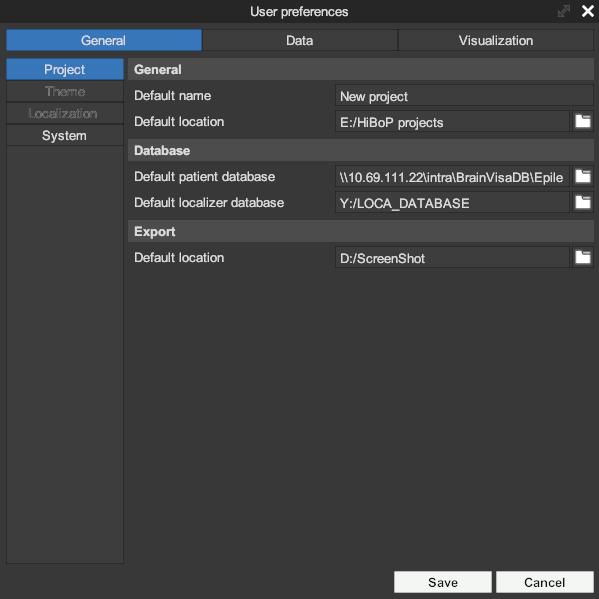
\includegraphics[scale=0.5]{Preferences.png}
\end{center}
\caption{\label{preferencesUI}Preferences}
\end{figure}
\begin{itemize}
\item \textbf{Default Name} : Default name for a new project
\item \textbf{Projects} : Default path to search for projects
\item \textbf{Patients} : Default path to patients database
\item \textbf{Localizers} : Default path to functional data
\item \textbf{Screenshots} : Default path to save screenshots
\item \textbf{Site name correction} : Change the name of a certain patern of site names (for instance "xp4" becomes "X'4")
\item \textbf{Automatic iEEG Update} : Update the iEEG values on the brain automatically if they are outdated
\item \textbf{Event position} : How to average the secondary events position
\item \textbf{Value} : How to average the values
\item \textbf{Type} : Show every matrices of a selected protocol or only blocs chosen in columns
\item \textbf{Smoothing} : Should the matrices be smoothed horizontally (to have a better resolution)
\item \textbf{Normalization by baseline} : The following formula is applied to each value $v$ $$v = \frac{v - \mu_{b}}{\sigma_{b}}$$ where $b$ is an array of the baseline values depending on this parameter, $\mu_b$ is their mean and $\sigma_b$ is their standard deviation
\item \textbf{Bloc format} : How the trial matrices should be displayed (parameters depend on this parameter, try yourself to see which one is better for you)
\item \textbf{Trial synchronization} : Should the matrices be synchronized when selecting specific trials
\item \textbf{Theme} : Theme of the software (light theme is still under development)
\item \textbf{Cut lines} : Should the cut lines appear on the cuts ?
\item \textbf{Hide curve when column hidden} : Should the curves of the hidden column appear ?
\end{itemize}
\subsection{Project management}
\subsubsection{Creating, opening and saving a project}
\paragraph{} When creating a new project, you have to specify the name of your new project, the location where it will be saved, the location of the anatomical database and the location of the functional database (Figure \ref{newProjectUI}). The two last fields are optional.
\begin{figure}[H]
\begin{center}
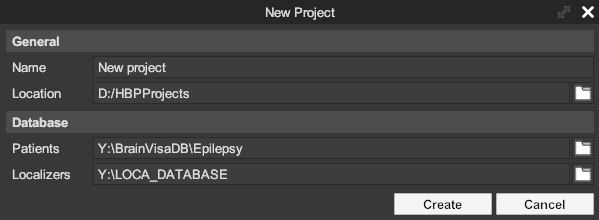
\includegraphics[scale=0.5]{NewProject.png}
\end{center}
\caption{\label{newProjectUI}Create a new project}
\end{figure}
\paragraph{} In order to open a previously created project (Figure \ref{openProjectUI}), you have to tell where your projects are located. Once these are loaded, you can either double click on the project you want to open or select the project and then click on Open. You can also sort projects using specific parameters.
\begin{figure}[H]
\begin{center}
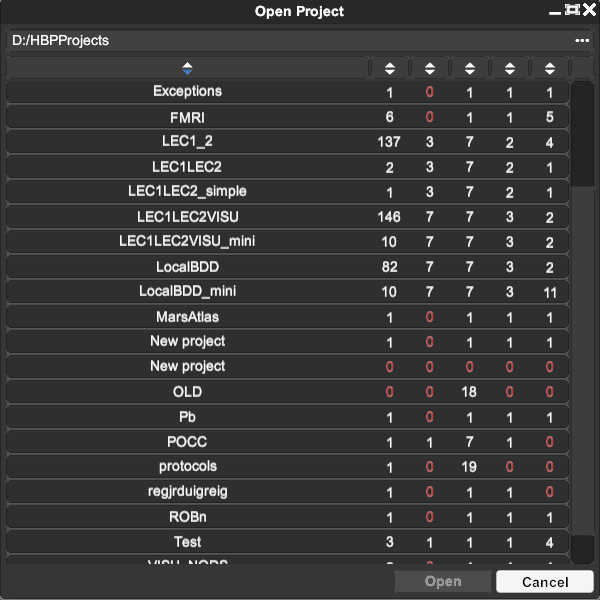
\includegraphics[scale=0.5]{OpenProject.png}
\end{center}
\caption{\label{openProjectUI}Open a project}
\end{figure}
\paragraph{} If you want to save a project to a different location or with a different name than when it was open, you can use the "Save as" menu (Figure \ref{saveProjectUI}).
\begin{figure}[H]
\begin{center}
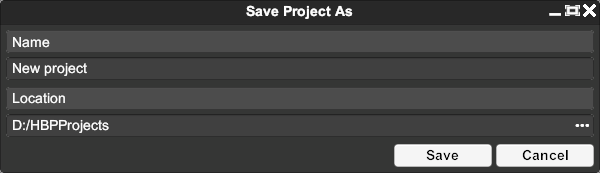
\includegraphics[scale=0.5]{SaveAs.png}
\end{center}
\caption{\label{saveProjectUI}Save a project as}
\end{figure}
\paragraph{} All of these menus are located in the File menu at the top of the screen.
\subsubsection{Patients management}
\paragraph{} To add patients to the opened project, you have to use the patients manager (Figure \ref{patientGestionUI}). The window has two panels: the left panel displays all available patients in the database (found in the folder you specify at the top of the window) whereas the right panel displays patients added to this project. For each patient, numbers indicate the status of their respective anatomical data (Meshes, MRIs, Implantations and Connectivities). To add or remove patients, you can either select them in any list and use the arrows to add or remove them, or you can create new patients from scratch using the "+" button in the center. In order for the anatomical database to be correctly loaded, you have to use a specific hierarchy described in appendix \ref{bddhierarchy}.
\begin{figure}[H]
\begin{center}
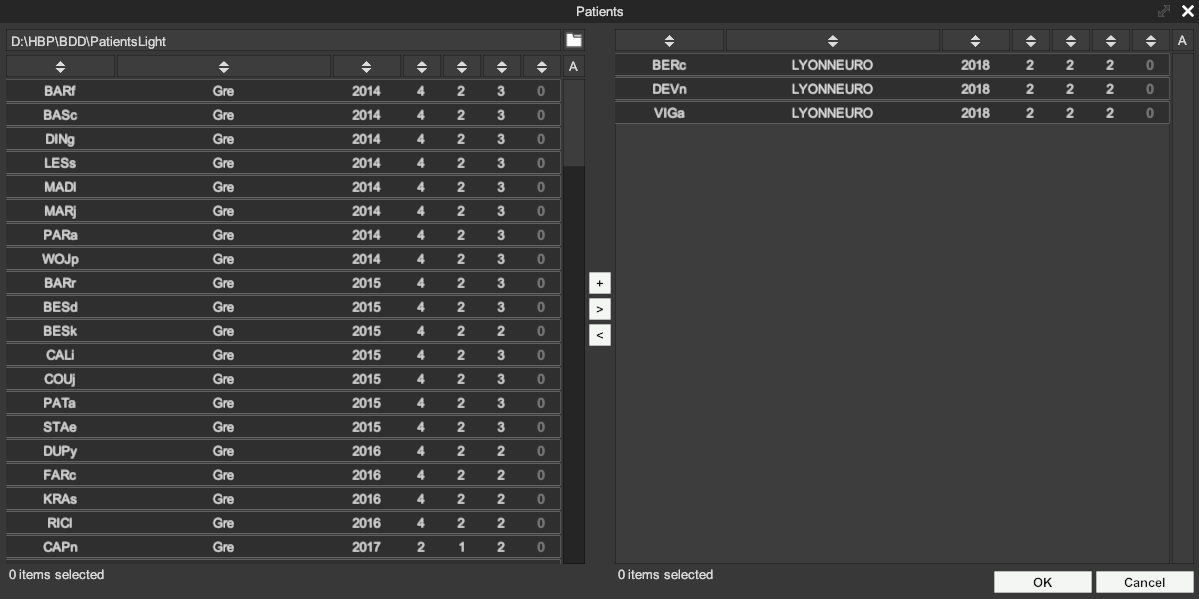
\includegraphics[scale=0.3]{PatientGestion.png}
\end{center}
\caption{\label{patientGestionUI}Patients manager}
\end{figure}
\paragraph{} To edit any loaded patient, you can double click\footnote{The process of double clicking an item to edit it is common to most windows of HiBoP} on it. This will open the patient modifier window (Figure \ref{patientModifierUI}) which will allow you to edit anything concerning the metadata or the anatomical data of this patient. You can navigate between anatomical data types using the tabs in the middle of the window.
\begin{figure}[H]
\begin{center}
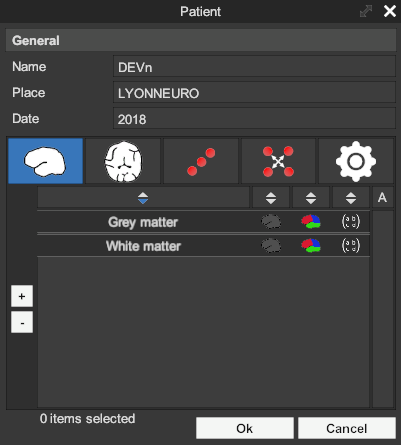
\includegraphics[scale=0.5]{PatientModifier.png}
\end{center}
\caption{\label{patientModifierUI}Patient modifier}
\end{figure}
\paragraph{} If you want to add a mesh, you can use the "+" button located to the left; if you want to edit a mesh, you can double click the mesh item, and this will open a mesh modifier window (Figure \ref{meshModifierUI}) which will allow you to edit the path to the GIfTI files or to the transformation file.
\begin{figure}[H]
\begin{center}
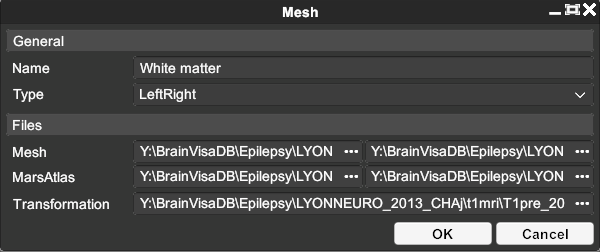
\includegraphics[scale=0.5]{MeshModifier.png}
\end{center}
\caption{\label{meshModifierUI}Mesh modifier}
\end{figure}
\paragraph{} As stated in section \ref{data}, you can also create groups of patients to add them more easily to the visualizations. This is done through the groups manager window (Figure \ref{groupGestionUI}). To create a new group, use the "+" button on the left. To remove existing groups, select the group(s) you want to remove, and use the "-" button on the left\footnote{The process of using "+" button to add and "-" button to remove is common to most windows of HiBoP}. Adding and removing patients from a group is very similar to the patients manager window (Figure \ref{groupModifierUI}).
\begin{figure}[H]
\begin{center}
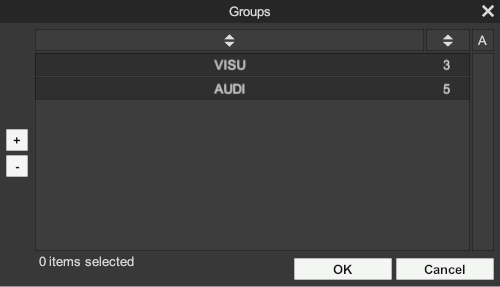
\includegraphics[scale=0.5]{GroupGestion.png}
\end{center}
\caption{\label{groupGestionUI}Groups manager}
\end{figure}
\begin{figure}[H]
\begin{center}
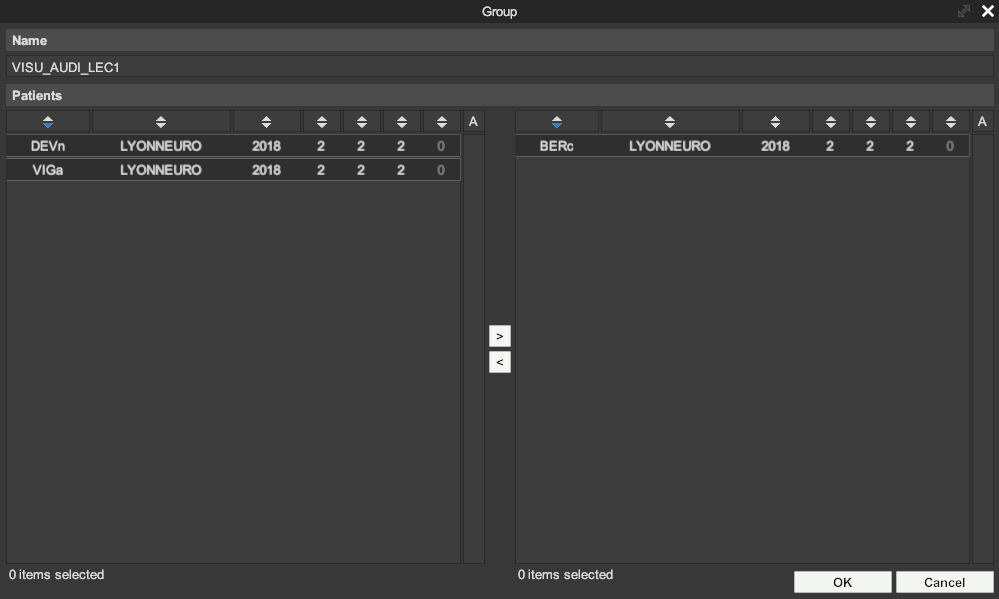
\includegraphics[scale=0.3]{GroupModifier.png}
\end{center}
\caption{\label{groupModifierUI}Group modifier}
\end{figure}
\subsubsection{Data management}
\begin{figure}[H]
\begin{center}
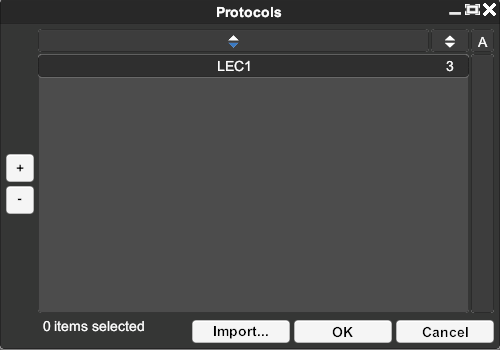
\includegraphics[scale=0.5]{ProtocolGestion.png}
\end{center}
\caption{\label{protocolGestionUI}Protocols manager}
\end{figure}
\begin{figure}[H]
\begin{center}
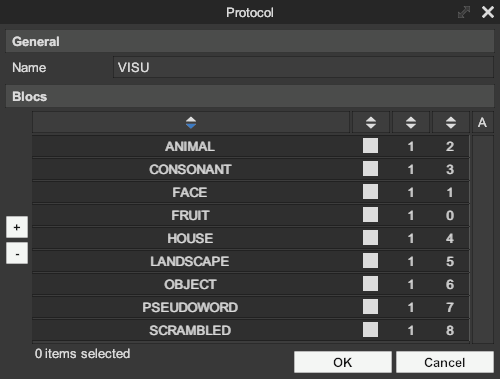
\includegraphics[scale=0.3]{ProtocolModifier.png}
\end{center}
\caption{\label{protocolModifierUI}Protocol modifier}
\end{figure}
\begin{figure}[H]
\begin{center}
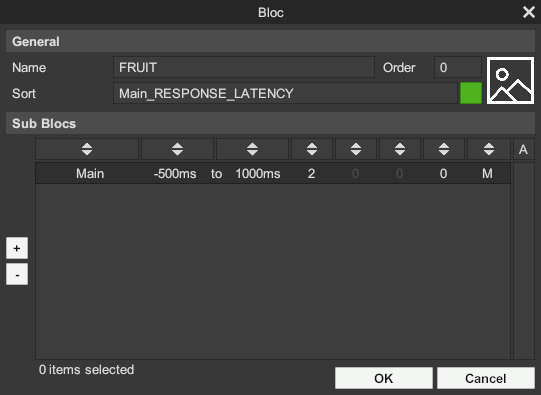
\includegraphics[scale=0.5]{BlocModifier.png}
\end{center}
\caption{\label{blocModifierUI}Bloc modifier}
\end{figure}
\begin{figure}[H]
\begin{center}
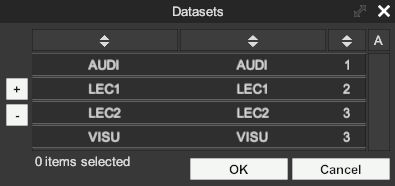
\includegraphics[scale=0.5]{DatasetGestion.png}
\end{center}
\caption{\label{datasetGestionUI}Datasets manager}
\end{figure}
\begin{figure}[H]
\begin{center}
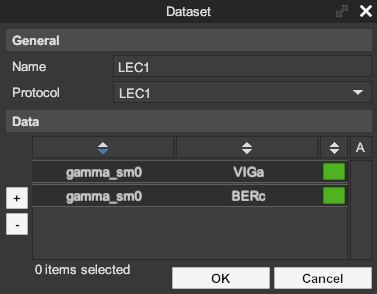
\includegraphics[scale=0.5]{DatasetModifier.png}
\end{center}
\caption{\label{datasetModifierUI}Dataset modifier}
\end{figure}
\begin{figure}[H]
\begin{center}
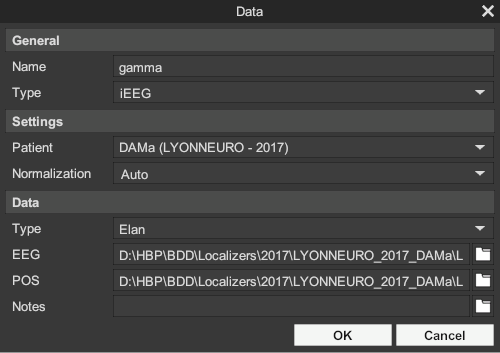
\includegraphics[scale=0.5]{DataInfoModifier.png}
\end{center}
\caption{\label{dataInfoModifierUI}Data information modifier}
\end{figure}
\subsubsection{Visualizations management}
\appendix
\section{HiBoP Database Manager}\label{bddmanager}
\section{HiBoP Database Hierarchy}\label{bddhierarchy}
\end{document}